\documentclass{article}


\usepackage{graphicx}
\usepackage{float}
%\usepackage{sidecap}
%\usepackage{csquotes} % ещё одна штука для цитат
\newtheorem{theorem}{Определение} % чтобы заработало окружение теорем

\usepackage[T2A]{fontenc}
\usepackage[utf8]{inputenc}
\usepackage[russian]{babel}
\usepackage{enumerate}
\usepackage{amsmath}

\newcommand{\rom}[1]
    {\MakeUppercase{\romannumeral #1}}

\usepackage{graphicx}
\title{Линейная Алгебра}
\author{Панов Петр Алексеевич}
\begin{document}
\maketitle
 
\tableofcontents

\section*{Структура курса}
\begin{itemize}
\item 3-4 модуль 1 курса
\begin{itemize}
\item КР - начало 4 модуля(0.3)
\item Экзамен - конец 4 модуля(0.5)
\item Текущая успеваемость - квизы, самостоятельные и т.д (0.2)

Можно компенсировать это выходом к доске, если проспал или плохо написал. Как работает разбалловка внутри этого пункта - одному Панову известно. Скорее всего, все СР+2 выхода к с доске=100\%.
\end{itemize}

\item 1-2 модуль 2 курса
\begin{itemize}
\item КР - начало 2 модуля(0.3)
\item Экзамен - конец 2 модуля(0.5)
\item Текущая успеваемость - квизы, самостоятельные и т.д (0.2)
\end{itemize}
\item итоговая оценка - среднее арифметическое итогов 1 курса и 2 курса.
\end{itemize}

Блоков нет, все можно переписать, если по уважительной причине прогулял - перед сессией.С неуважительными причинами - нельзя.

Материалы - в ЛМС.

\section*{Книги}
\begin{itemize}
\item Бурмистрова Лобанов - 1 часть
\item Хованская ирина Аскольдовна - курс на Курсере
\end{itemize}

\section*{Введение}
Линейная алгебра изучает линейные пространства. Что это - пока не скажем, но к ним откосятся множество действительных и мнимых чисел, матриц и векторов.
\subsection*{Комплексные числа}
Это такие числа, которые содержат помимо действительной, еще и мнимую часть. Мнимая единица $i$ - число, такое, что $i^2=-1$. 
Соответственно, комплексное число имеет вид $a+bi$, $a$ - действительная часть, $b$ - мнимая.
Рассмотрим их свойства.

$$Z_1 = a_1 + b_1i, Z_2 = a_2 + b_2i$$
$$Z_1+Z_2 = (a_1+a_2) + (b_1+b_2)i$$
$$Z_1-Z_2 = (a_1-a_2) + (b_1-b_2)i$$
$$Z_1*Z_2 = (a_1a_2-b_1b_2) + (b_1a_2+a_1b_2)i$$
$$Z_1/Z_2 = \frac{a_1+b_1i}{a_2+b_2i} = \frac{(a_1+b_1i)(a_2-b_2i)}{a_2^2+b_2^2} = \frac{(a_1a_2+b_1b_2)}{a_2^2+b_2^2} + \frac{(b_1a_2-a_1b_2)i}{a_2^2+b_2^2}$$

Также комплексное число можно рассмотреть как точку на плоскости, аналогично тому, как действительное как точку на прямой. 
Точке (1023;65536) соответствует число $1023+65536 i $, например. 

Модуль комплексного числа определен как длинна радиус-вектора, направленного из нуля в соответствующую точку и равен $\sqrt{a^2 + b^2}$.

Аргумент комплексного числа($Arg(Z) = \varphi$) - это угол между осью x и радиус-вектором этого числа. 
Ясно, что $\sin \varphi = \frac y{|Z|}$, $\cos \varphi = \frac x{|Z|}$, $\tan \varphi = \frac yx$

Еще один способ представления - через число  $e$:

    $$z = r (\cos \varphi + i \sin \varphi )$$ 
    
Еще один способ дает формула Эйлера:

    $$e ^{i\varphi}= cos \varphi + i sin \varphi$$
    
где $e$ — число Эйлера
Применяя эту формулу к тригонометрической форме, получим показательную форму комплексного числа:

    $$z = r e ^{i \varphi}$$
   
Следствия
\begin{itemize}
    \item Модуль выражения $e^{i\varphi}$,  где $\varphi$ вещественно, равен 1.
    \item $ \cos \varphi =\frac {e^{i\varphi }+e^{-i\varphi }}{2}$, 
    $ \sin \varphi =\frac {e^{i\varphi }-e^{-i\varphi }}{2i}$
\end{itemize}

Степени и корни:

$$ z^{n}=\left[r\left(\cos \varphi +i\sin \varphi \right)\right]^{n}=r^{n}\left(\cos n\varphi +i\sin n\varphi \right)$$,

$$z^{1/n}=\left[r\left(\cos \left(\varphi +2\pi k\right)+i\sin \left(\varphi +2\pi k\right)\right)\right]^{1/n}={\sqrt[{n}]{r}}\left(\cos {\frac {\varphi +2\pi k}{n}}+i\sin {\frac {\varphi +2\pi k}{n}}\right),\quad k=0,\;1,\;\ldots ,\;n-1.$$

Так что существуют корни любой степени, а их число равно степени.


\section*{Линейные преобразования}

Линейное преобразование - это преобразование, которое каждому элементу $R^n$ ставит элемент этого же $R^n$, причем $\varphi(a+b) = \varphi(a) + \varphi(b)$. 

На примере векторов из двух элементов:

$\varphi: (a,b) \to (3a, -5b)$ - линейное преобразование.
$\varphi: (a,b) \to (6a^3, b^7)$ - НЕ линейное преобразование

Каждое ЛП задается матрицей, и каждая матрица соответствует какому-то ЛП.

\subsection*{Матрицы}

$$A=\begin{pmatrix}
a_{11}  &a_{12}  &\cdots  &a_{1n} \\
a_{21}  &a_{22}  &\cdots  &a_{2n} \\
\vdots  &\vdots  &\ddots  &\vdots \\
a_{m1}&a_{m2}&\cdots  &a_{mn}
\end{pmatrix}$$

Для матрицы определены следующие алгебраические операции:
\begin{itemize}
    \item сложение матриц, имеющих один и тот же размер;
    \item умножение матриц подходящего размера (матрицу, имеющую $n$ столбцов, можно умножить справа на матрицу, имеющую $n$строк);
    \item в том числе умножение на матрицу вектора (по обычному правилу матричного умножения; вектор является в этом смысле частным случаем матрицы);
    \item умножение матрицы на скаляр.
\end{itemize}

\subsubsection*{Сложение матриц}

Складывать можно только матрицы одинакового размера.

Сложение матриц  $A+B$ есть операция нахождения матрицы $C$, все элементы которой равны попарной сумме всех соответствующих элементов матриц $A$ и $B$, то есть каждый элемент матрицы $C$ равен

      $$ c_{ij} = a_{ij} + b_{ij}$$

Свойства сложения матриц:
\begin{itemize}
    \item коммутативность: $A+B = B+A$;
    \item ассоциативность: $(A+B)+C =A+(B+C)$;
    \item сложение с нулевой матрицей: $A + \Theta = A$;
    \item существование противоположной матрицы: $A + (-A) = \Theta$;
\end{itemize}

\subsubsection*{Умножение матрицы на число}

Умножение матрицы $A$ на число $\lambda \in R$ заключается в построении матрицы $\lambda A = ( \lambda a_{ij} )$.



Свойства умножения матриц на число:
\begin{itemize}
    \item умножение на единицу: $1A = A$;
    \item ассоциативность: $(\lambda\beta)A = \lambda(\beta A)$;
    \item дистрибутивность: $(\alpha+\beta)A = \alpha A + \beta A$;
    \item дистрибутивность: $\alpha(A+B) = \alpha A + \alpha B$;
\end{itemize}

\subsubsection*{Умножение матриц}
\begin{figure}
  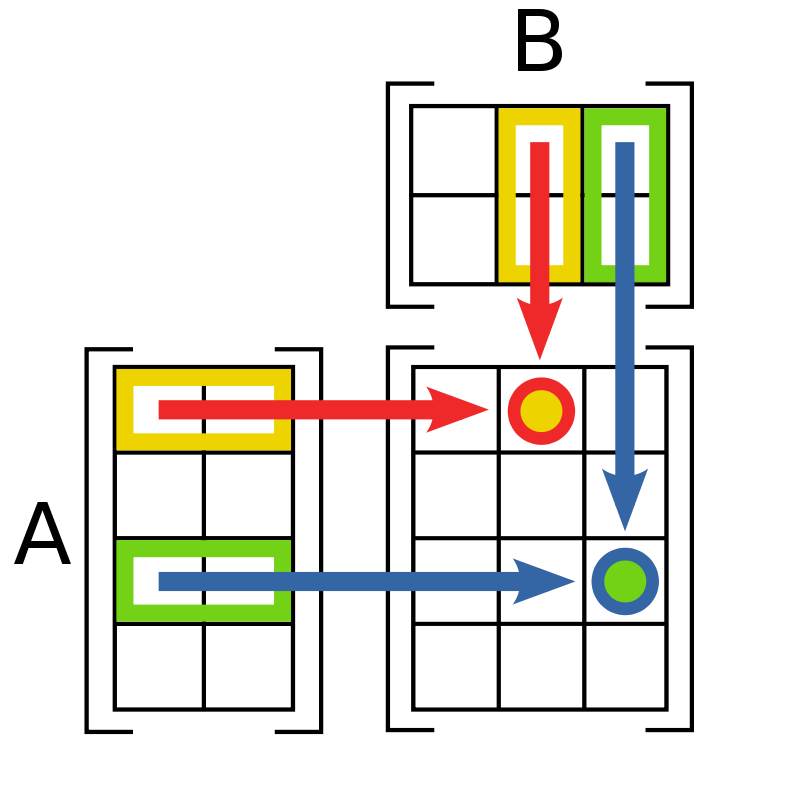
\includegraphics[width=0.6\linewidth]{matrix-multiplication.png}
  \caption{Умножение матриц}
\end{figure}
Умножение матриц (обозначение: $AB$, реже со знаком умножения $A\times B$ — есть операция вычисления матрицы $C$,
каждый элемент которой равен сумме произведений элементов в соответствующей строке первого множителя и столбце второго.

$$c_{ij}=\sum _{k=1}^{n}a_{ik}b_{kj}$$

Количество столбцов в матрице $A$ должно совпадать с количеством строк в матрице $B$, иными словами, 
матрица $A$ обязана быть согласованной с матрицей $B$. 
Если матрица $A$ имеет размерность $m\times n$, $B$ - $ n\times k$, 
то размерность их произведения $AB=C$ есть $m\times k$.

Свойства умножения матриц:

\begin{itemize}
    \item ассоциативность: $(AB)C = A(BC)$;
    \item некоммутативность (в общем случае): $AB \neq BA$;
    \item произведение коммутативно в случае умножения с единичной матрицей: $AI = IA$;
    \item дистрибутивность: $(A+B)C = AC + BC$, $A(B+C) = AB + AC$;
    \item ассоциативность и коммутативность относительно умножения на число: $(\lambda A)B = \lambda (AB) = A(\lambda B)$;
\end{itemize}

Для квадратных матриц существует единичная матрица $E$ (аналог единицы для операции умножения чисел) такая,
что умножение любой матрицы на неё не влияет на результат, а именно $EA=AE=A$

У единичной матрицы единицы стоят только по главной диагонали, остальные элементы равны нулю
$$E=\begin{pmatrix}1&0&\cdots &0\\0&1&\cdots &0\\\vdots &\vdots &\ddots &\vdots \\0&0&\cdots &1\end{pmatrix}$$

\subsection*{Собственные векторы}

Если $Av = \lambda v$, то вектор $v$ для матрицы $A$ - собственный.

\subsection*{Обратные матрицы}
Обратная матрица — такая матрица 

$A^{-1}$, 

при умножении на которую исходная матрица $A$ 
даёт в результате единичную матрицу $E$:

$$AA^{-1}=A^{-1}A=E$$

Методов расчета много, пока они не нужны.

\subsection*{Транспонирование}

Транспонирование матрицы - запись каждой строки исходной матрицы в качестве столбца. Еще можно сказать, что это симметричное отражение отн. главной диагонали

Например,
$\begin{bmatrix}
1 & 2 \\
3 & 4 \\
\end{bmatrix}^{T} =\begin{bmatrix}1&3\\2&4\end{bmatrix}$

Матрица $A*A^T$ - всегда симметрична


\subsection*{След матрицы}
$$tr(A) = \sum_{i=1}^na_{ii}$$

$$tr(\alpha A + \beta B) = \alpha tr(A) + \beta tr(B)$$

$$tr(A) = tr(A^T)$$

$$tr(AB) = tr(BA)$$

$$tr(B^{-1}AB) = A$$

\subsection*{Получение матрицы преобразований}

Если для некоторого преобразования выполняется:

 $\begin{pmatrix}
	1\\
	0\\
\end{pmatrix}' = \begin{pmatrix}
	a_{11}\\
	a_{21}\\
\end{pmatrix}$, а 
$\begin{pmatrix}
	0\\
	1\\
\end{pmatrix}' = \begin{pmatrix}
	a_{12}\\
	a_{22}\\
\end{pmatrix}$, то 
$A_{\phi} = \begin{pmatrix}
	a_{11} & a_{12}\\
	a_{21} & a_{22}\\
\end{pmatrix}$

\subsection*{Детерминант aka определитель}
$$A = \begin{pmatrix}
	a & b\\
	c & d\\
\end{pmatrix}$$

$$\det A = ad-bc$$

Определитель матрицы можно вычислить по формуле:

$$\Delta =
\begin{vmatrix}
a_{11}&a_{12}&a_{13}\\
a_{21}&a_{22}&a_{23}\\
a_{31}&a_{32}&a_{33}
\end{vmatrix}
=a_{11}\begin{vmatrix}
a_{22}&a_{23}
\\a_{32}&a_{33}
\end{vmatrix}
-a_{12}\begin{vmatrix}
a_{21}&a_{23}
\\a_{31}&a_{33}
\end{vmatrix}
+a_{13}\begin{vmatrix}
a_{21}&a_{22}
\\a_{31}&a_{32}
\end{vmatrix}$$

Определитель матрицы $2\times2$ - это (ориентированная!)площадь такого параллелограмма, который натянут на векторы - столбцы матрицы. Для матрицы $3\times 3$ это объем соответствующего параллелепипеда.

$$\det E =1$$

Если в матрице есть два одинаковых столбца/строки, определитель равен нулю. 

При умножении на число, определитель тоже умножается на это число.

$$\det AB = \det A \times \det B$$

Перестановка двух строк или столбцов меняет знак определителя.

$$\det A^T = \det A$$

\subsubsection*{Правило треугольников}
\begin{figure}[htp]
\centering
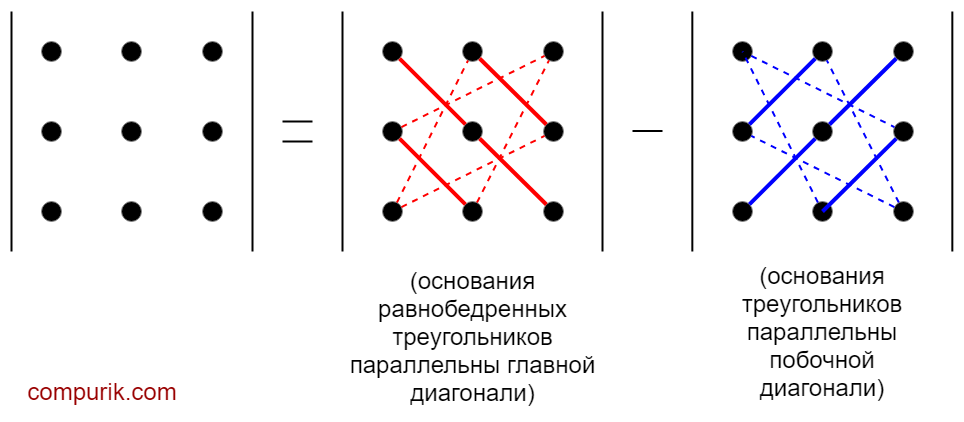
\includegraphics[scale=.400]{triangle.png}
\end{figure}

Правило треугольника позволяет более быстро посчитать определитель матрицы $3\times 3$. Можно еще приписать столбцы слева, и тройки параллельные главной диагонали брать с плюсом, перпендикулярные с минусом.


\subsection*{Алгебраическое дополнение}

Из матрицы вычеркиваем строку и столбец содержащие элемент $a_{ij}$, получаем алгебраическое дополнение этого элемента - $A_{ij}\times (-1)^{i+j}$. 

Можно посчитать определитель через алгебраические дполнения.

$$\det A = \sum_{i=1}^n a_{ij}A_{ij}(-1)^{i+j}$$

Такой метод называется раскрытием по строке(или столбцу). Ниже показан пример для матрицы $4\times 4$. Очевидно, выбирая строку/столбец надо выбирать тот(ту), где больше всего нулей.
\begin{figure}[htp]
\centering
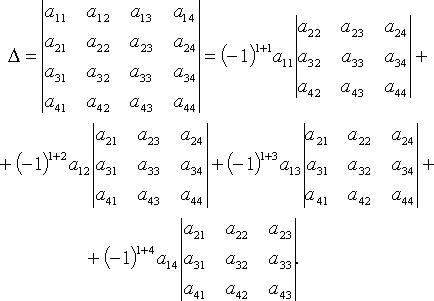
\includegraphics[scale=.600]{det-by-row.jpeg}
\end{figure}

Элементарное преобразование первого типа: строки в определителе можно менять местами. При нечетном числе смен меняется знак.

Сложение строк, умножение строк на число. Применяется в методе гаусса.

\subsection*{Обратная матрица}

$$A^{-1}A = E = AA^{-1}$$

$$\left(\begin{matrix}
	a & b\\
	c & d\\
\end{matrix}\right)^{-1} = 
\frac 1{ad-bc}\left(\begin{matrix}
	d & -b\\
	c & a\\
\end{matrix}\right)
$$

$$A^{-1} = \frac 1{|A|}(A_{ij})^T, i=1\ldots n, j=1 \ldots m$$

\subsection*{Матричные уравнения}

Обычную систему линейных уравнений можно записать так:

\begin{figure}[htp]
\centering
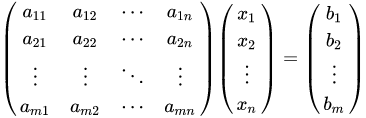
\includegraphics[scale=1.00]{linear-system.png}
\end{figure}

$$A\times x = B$$

а это более общий случай. Решить его можно так:

$$A^{-1}\times A \times x = A^{-1} \times B \Rightarrow x = A^{-1}B$$

Аналогично, если $x\times A = B$, то $x = b \times A^{-1}$

Пример:

$\begin{pmatrix}
	1 & 2\\
	3 & 4\\
\end{pmatrix} x = \begin{pmatrix}
	3 & 3\\
	5 & 7\\
\end{pmatrix}$

$A^{-1} = \frac 1{-2}\begin{pmatrix}
	4 & -2\\
	-3 & 1\\
\end{pmatrix} = \begin{pmatrix}
	-1 & 1\\
	\frac 32 & -\frac 12\\
\end{pmatrix}
$

$x =  \begin{pmatrix}
	-1 & 1\\
	\frac 32 & -\frac 12\\
\end{pmatrix} \times\begin{pmatrix}
	4 & -2\\
	-3 & 1\\
\end{pmatrix} = \begin{pmatrix}
	1 & -1\\
	1 & 2\\
\end{pmatrix}$




\end{document}



